
%(BEGIN_QUESTION)
% Copyright 2014, Tony R. Kuphaldt, released under the Creative Commons Attribution License (v 1.0)
% This means you may do almost anything with this work of mine, so long as you give me proper credit

Regn ut resistansen til strekklappen i denne målebro kretsen, gitt voltmeterets indikasjon på 5.6mV (A er positiv og B er negativ).

$$\includegraphics[width=15.5cm]{i00854x01.eps}$$

$R_{strain}$ = \underbar{\hskip 50pt}

\vfil 

\underbar{file i00854}
\eject
%(END_QUESTION)





%(BEGIN_ANSWER)

This is a graded question -- no answers or hints given!

%(END_ANSWER)





%(BEGIN_NOTES)

The voltmeter's indication of 5.8 millivolts (with A being more positive than B) tells us the strain gauge is dropping that much more voltage than the 4.7 k$\Omega$ resistor.  Our problem-solving strategy, therefore, will be to first calculate the voltage dropped by the 4.7 k$\Omega$ resistor, then add 5.8 mV to that value, and from that calculate $R_{strain}$.

\vskip 10pt

First, calculating voltage across the 4.7 k$\Omega$ resistor:

$$V_{4.7k} = 100 \hbox{ mV} \left(4700 \> \Omega \over {3300 \> \Omega + 4700 \> \Omega}\right) = 58.75 \hbox{ mV}$$

Now, calculating voltage across the strain gauge:

$$V_{strain} = 58.75 \hbox{ mV} + 5.8 \hbox{ mV} = 64.55 \hbox{ mV}$$

With the strain gauge dropping 64.55 mV, the 10 k$\Omega$ resistor must drop the remainder making up 100 mV (according to Kirchhoff's Voltage Law).  This means the 10 k$\Omega$ resistor must drop:

$$V_{10k} = 100 \hbox{ mV} - 64.55 \hbox{ mV} = 35.45 \hbox{ mV}$$

Ohm's Law will then tell us how much current is going through the 10 k$\Omega$ resistor, which is also the same current passing through the strain gauge:

$$I = {V \over R} = {35.45 \hbox{ mV} \over 10000 \> \Omega} = 3.545 \> \mu\hbox{A}$$

Now that we know both the current through the strain gauge (3.545 $\mu$A) and the voltage across it (64.55 mV), we may use Ohm's Law to calculate its resistance:

$$R_{strain} = {V \over I} = {64.55 \hbox{ mV} \over 3.545 \> \mu\hbox{A}} = 18.21 \hbox{ k}\Omega$$

%INDEX% Electronics review: Kirchhoff's Voltage Law (KVL)
%INDEX% Electronics review: series-parallel circuits
%INDEX% Measurement, strain gauge

%(END_NOTES)

